\documentclass[tikz]{standalone}

\usetikzlibrary{arrows.meta,positioning}

\begin{document}
	\setlength{\baselineskip}{16pt}
	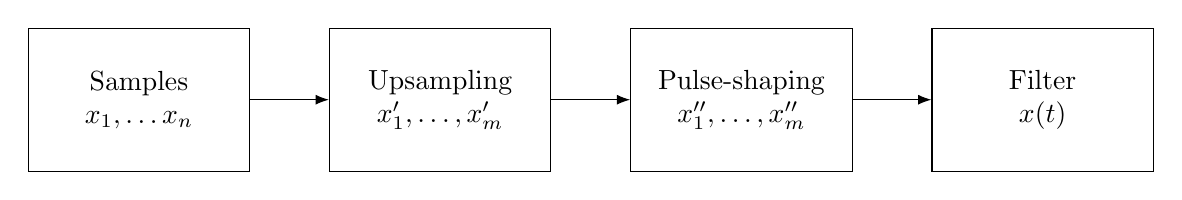
\begin{tikzpicture}[
		block/.style={draw, align=center, minimum height=12ex, minimum width=8em}
	]
		\node[block] (spl) {Samples\\$x_1,\dots x_n$};
		\node[block, right=of spl] (ups) {Upsampling\\$x_1^\prime,\dots,x_m^\prime$};
		\node[block, right=of ups] (pls) {Pulse-shaping\\$x_1^{\prime\prime},\dots,x_m^{\prime\prime}$};
		\node[block, right=of pls] (flt) {Filter\\$x(t)$};

		\draw[-Latex] (spl) -- (ups);
		\draw[-Latex] (ups) -- (pls);
		\draw[-Latex] (pls) -- (flt);
	\end{tikzpicture}
\end{document}